% vim:spell:spelllang=en

%\newcommand{\var}[1]{\ensuremath{\mathtt{#1}}}


\chapter{SSA Reconstruction \Author{S. Hack}}
\inputprogress
\label{chapter:repair_maintain_ssa_after_optimization}
\graphicspath{{repair_maintain_ssa_after_optimization/}{part1/repair_maintain_ssa_after_optimization/}}


%Here the currssadir is \currentssadir.

\section{Introduction}

Some optimizations break the single-assignment property of the SSA form by inserting additional definitions for a single SSA value.
A common example is live-range splitting by inserting copy operations or inserting spill and reload code during register allocation.
Other optimizations, such as loop unrolling or jump threading, might duplicate code, thus adding additional variable definitions, \emph{and} modify the control flow of the program.
We will first go through two examples before we present algorithms to properly repair SSA.

\subsection{Live-Range Splitting}

The first example is depicted in Figure~\ref{fig:ex1}.
Our spilling pass decided to spill a part of the live range of variable $x_0$ 
in the right block in~\subref{sfig:harmless}, resulting in the code shown 
in~\subref{sfig:nonssa},
where it inserted a store and a load instruction. 
This is indicated by assigning to the memory location $X$.
The load is now a second definition of $x_0$, violating the SSA form that has 
to be reconstructed as shown in~\subref{sfig:recons}.
This example shows that maintaining SSA also involves placing new \phifuns.

\begin{figure}[htbp]
	\centering
	\subfloat[Original program] {
		\label{sfig:harmless}
                \tikzsubfigure[1]{spill}
		% \input spill_orig.tikz
	}
	\hfill
	\subfloat[Spilling~$x_0$, SSA broken] {
		\label{sfig:nonssa}
                \tikzsubfigure[2]{spill}
	}
	\hfill
	\subfloat[SSA reconstructed] {
		\label{sfig:recons}
                \tikzsubfigure[3]{spill}
	}
	\caption{Adding a second definition as a side-effect of spilling.}
	\label{fig:ex1}
\end{figure}

Many optimizations perform such program modifications, and 
maintaining SSA is often one of the more complicated and error-prone parts in 
such optimizations, owing to the insertion of additional \phifuns and the 
correct redirection of the uses of the variable.

\subsection{Jump Threading}

Jump threading is a transformation performed by many popular compilers such as GCC and LLVM.
It partially evaluates branch targets to save branches and provide more context to other optimizations.
Consider the situation where
a block contains a conditional branch that depends on some variable \var x.
In the example shown in Figure~\ref{fig:threading}, the conditional branch tests if $\var x> 0$.

Assume that the block containing that conditional branch has multiple predecessors and \var x can be proven constant for one of the predecessors.
In our example, this is shown by the assignment $\var x_1\gets~0$. 
Jump threading now partially evaluates the conditional branch by directly making the corresponding successor of the branch block a successor of the \emph{predecessor} of the branch.
To this end, the code of the branch block is duplicated and attached to the predecessor. 
This also duplicates potential definitions of variables in the branch block.
Hence, SSA is destroyed for those variables and has to be reconstructed. 
However, in contrast to the previous spill example, the control flow has 
changed which poses an additional challenge for an efficient SSA reconstruction 
algorithm. 

\begin{figure}[htbp]
  \begin{center}
    \subfloat[Original program]{
    \tikzsubfigure[1]{jump_threading}
    }
    \hfill
    \subfloat[Jump threaded]{
    \tikzsubfigure[2]{jump_threading}
    }
    \hfill
    \subfloat[SSA reconstructed]{
    \tikzsubfigure[3]{jump_threading}
    }
  \end{center}
  \caption{Jump Threading can break SSA, which has to be reconstructed.}
  \label{fig:threading}
\end{figure}


\section{General Considerations}
In this chapter, we will discuss two algorithms.
The first is an adoption of the classical dominance-frontier based algorithm.
The second performs a search from the uses of the variables to the definition and places \phifuns on demand at appropriate places. 
In contrast to the first, the second algorithm might not construct minimal SSA 
form in general;
However, it does not need to update its internal data structures when the CFG is modified. 

We consider the following scenario: The program is represented as a control flow graph (CFG) and is in SSA form with dominance property.
For the sake of simplicity, we assume that each instruction in the program only writes to a single variable.
%Due to the single assignment property of the SSA form, we can identify the program point of the instruction and the variable. 
An optimization or transformation violates SSA by inserting additional definitions for an existing SSA variable, like in the examples above.
The original variable and the additional definitions can be seen as a single non-SSA variable that has multiple definitions and uses.

In the following, $v$ will be such a non-SSA variable.
Before reconstructing SSA for~$v$, every definition of~$v$ is numbered. 
This establishes the single-assignment property. 
What remains is associating every use of~$v$ with a suitable definition.
In the pseudocode \verb|v.defs| denotes the set of all SSA variables that represent~$v$.
A use of a variable is a pair consisting of a program point (a variable) and an integer denoting the index of the operand at the using instruction.

Both algorithms presented in this chapter share the same driver routine (Algorithm~\ref{alg:ssaconstr_driver}).
First, for every basic block~\verb|b| we compute a list~\verb|b.defs| that contains all instructions in the block which define one of the variables in~\verb|v.defs|.
This list is sorted according to the schedule of the instructions in the block from back to front.
Hence, the latest definition is the first in the list.

Then, all uses of the variable~$v$ are scanned.
Here we have to differentiate whether the user is a \phifun or not.
If it is, the variable's use occurs at the end of the predecessor block that corresponds to the position of the variable in the $\phi$'s argument list.
In that case, we start looking for the reaching definition at the end of that block.
Otherwise, we scan the block's list backwards until we find the first definition in front of the use.
If there is no such definition, we have to find one that reaches this block from \emph{outside.}
We use two functions \verb|find_def_from_begin| and \verb|find_def_from_end| that find the reaching definition at the beginning and end of a block, respectively. 
Algorithm~\ref{alg:ssaconstr_driver} shows that \verb|find_def_from_end| can be expressed in terms of \verb|find_def_from_begin|. 
\verb|find_def_from_end| additionally considers definitions in the block, while \verb|find_def_from_begin| does not.
Our two approaches only differ in the implementation of the function \verb|find_def_from_begin|.
The differences are described in the next two sections.
\begin{algorithm}
	\caption{SSA Reconstruction Driver}
	\label{alg:ssaconstr_driver}

\begin{verbatim}
proc ssa_reconstruct(variable v):
  for d in v.defs:
    b = d.block
    insert d in b.defs according to schedule
    # latest definition is first in list

  for each use (u, index) of v:
    d = None
    b = u.block
    if u.is_phi():
      b = u.block.pred(index)
      d = find_def_from_end(b)
    else:
      for l in b.defs:
        if l.order < u.order:
          d = l
          break
      # no local definition was found, search in the predecessors
      if not d:
        d = find_def_from_begin(b)

    rewrite use at u to d

proc find_def_from_end(block b):
  if not b.defs.empty():
    return b.defs[0]
  return find_def_from_begin(b)
\end{verbatim}
\end{algorithm}
%proposed by Sastry and Ju~\cite{sastry98}, 
\section{Reconstruction based on the Dominance Frontier}
This algorithm follows the same principles as the classical SSA construction algorithm by Cytron at al.~as described in chapter~(TODO: reference to the chapter).
We compute the iterated dominance frontier (IDF) of~$v$.
This set is a sound approximation of the set where \phifuns must be placed (it might contain blocks where a \phifun would be dead).
Then, we search for each use~$u$ the corresponding reaching definition.
This search starts at the block of~$u$.
If that block is in the IDF of~$v$ a \phifun needs to be placed at its entrance.
This \phifun has to be inserted into the list of definitions of~$v$ in that block.
The operands of the newly created \phifun will query their reaching definitions by recursive calls to \verb|find_def_from_end|.
The operands of that \phifun are then (recursively) searched in the predecessors of the block.
Because we inserted the \phifun into the \verb|b.defs| \emph{before} searching for the arguments, no infinite recursion can occur.
If the block is not in the IDF, the search continues in the block's immediate dominator. 
This is because in SSA, every use of a variable must be dominated by its definition\footnote{The definition of an operand of a \phifun has to dominate the according predecessor block.}.
Therefore, the reaching definition is the same for all predecessors and hence for the immediate dominator of this block.
Algorithm~\ref{alg:ssaconstr} shows this procedure in pseudo-code.

\begin{algorithm}
  \caption{SSA Reconstruction based on Dominance Frontiers}
  \label{alg:ssaconstr}
\begin{verbatim}
proc find_def_from_begin(block b):
  if b in IDF:
    d = new_phi(b)
    b.defs.append(d)
    i = 0
    for p in b.preds: 
      o = find_def_from_end(p, IDF)
      set i-th operand of d to o
      i = i + 1
  else:
    d = find_def_from_end(b.idom)
  return d
\end{verbatim}
\end{algorithm}

\section{Search-based Reconstruction}

The second algorithm we present here is similar to the construction algorithm that Click describes in his thesis~\cite{click:thesis}.
Although his algorithm is designed to construct SSA from the abstract syntax tree, it also works well on control flow graphs.
Its major advantage over the algorithm presented in the last section is that it does neither require dominance information nor dominance frontiers.
Thus it is well suited to be used in transformations that change the control flow graph.
Its disadvantage is that potentially more blocks have to be visited during the reconstruction.
The principle idea is to start a search from every use to find the corresponding definition, inserting \phifuns on the fly, while caching the found definitions at the basic blocks.
As in the last section, we only consider the reconstruction for a single variable called~$v$ in the following.
If multiple variables have to be reconstructed, the algorithm can be applied to each variable separately.

We perform a backward depth-first search in the CFG to collect the reaching definitions of the variable in question at each block.
We record the SSA variable that corresponds to the reaching definition of~$v$ at the end of the block in the field \verb|def| of the block.
If the CFG is a DAG, all predecessors of a block can be visited before the block itself is processed (post-order traversal).
Hence, all definitions that reach~\verb|b| can be computed before we decide whether to place a \phifun in~\verb|b| or not.
If more than one definition reaches the block, we need to place a \phifun.

If the CFG has loops, there are blocks for which not all reaching definitions can be computed before we can decide whether a \phifun has to be placed.
Recursively computing the reaching definitions for a block~\verb|b| can end up at~\verb|b| itself.
To avoid infinite recursion, we create a \phifun \verb|phi| without operands in the block before descending to the predecessors. 
Hence, if a variable has no definition in a loop, the \phifun placed in the header eventually reaches itself (and can later be eliminated). 
When we return to~\verb|b| we decide whether a \phifun has to be placed in~\verb|b| by looking at the reaching definition for every predecessor.
If the set of reaching definitions is a subset of $\{w,x\}$ where~$x$ is the \phifun inserted at~\verb|b| and~$w$ some other variable, then the \phifun is not necessary and we can propagate~$w$ further downwards.
In Algorithm~\ref{alg:ssaconstr_click}, this check is done by the function \verb|phi_necessary|.

\begin{algorithm}
	\caption{Search-based SSA Reconstruction}
	\label{alg:ssaconstr_click}

\begin{verbatim}
proc find_def_from_begin(block b):
  if b.def != None:
    return b.def
  pending = make_phi()
  reaching_defs = []
  for p in b.preds:
    reaching_defs += find_def_from_end(p)
  definite = phi_necessary(pending, reaching_defs)
  if pending == definite:
    set_arguments(definite, reaching_defs)
  b.def = definite
  return definite

# checks, if the parameter list in reaching_defs makes a phi function 
# necessary. This is the case if it is a subset of { other, pending_phi }
proc phi_necessary(variable pending_phi, list of variables reaching_defs):
  other = None
  for d in reaching_defs:
    if d == pending_phi:
      continue
    if other == None:
      other = d
    elif other != d:
      return pending_phi
  # this assertion is violated if reaching_defs only contains pending_phi
  # which never can happen
  assert other != None
  return other
  
\end{verbatim}
\end{algorithm}

In programs with loops, it can be the case that the local optimization which Algorithm~\ref{alg:ssaconstr_click} performs by calling \verb|phi_necessary| does not remove all unnecessary \phifuns. 
This can happen in loops where \phifuns can become unnecessary because other \phifuns are optimized away. 
Consider the example in Figure~\ref{fig:phiopt}.
\begin{figure}[htbp]
	\begin{center}
		\subfloat[Original program] {
			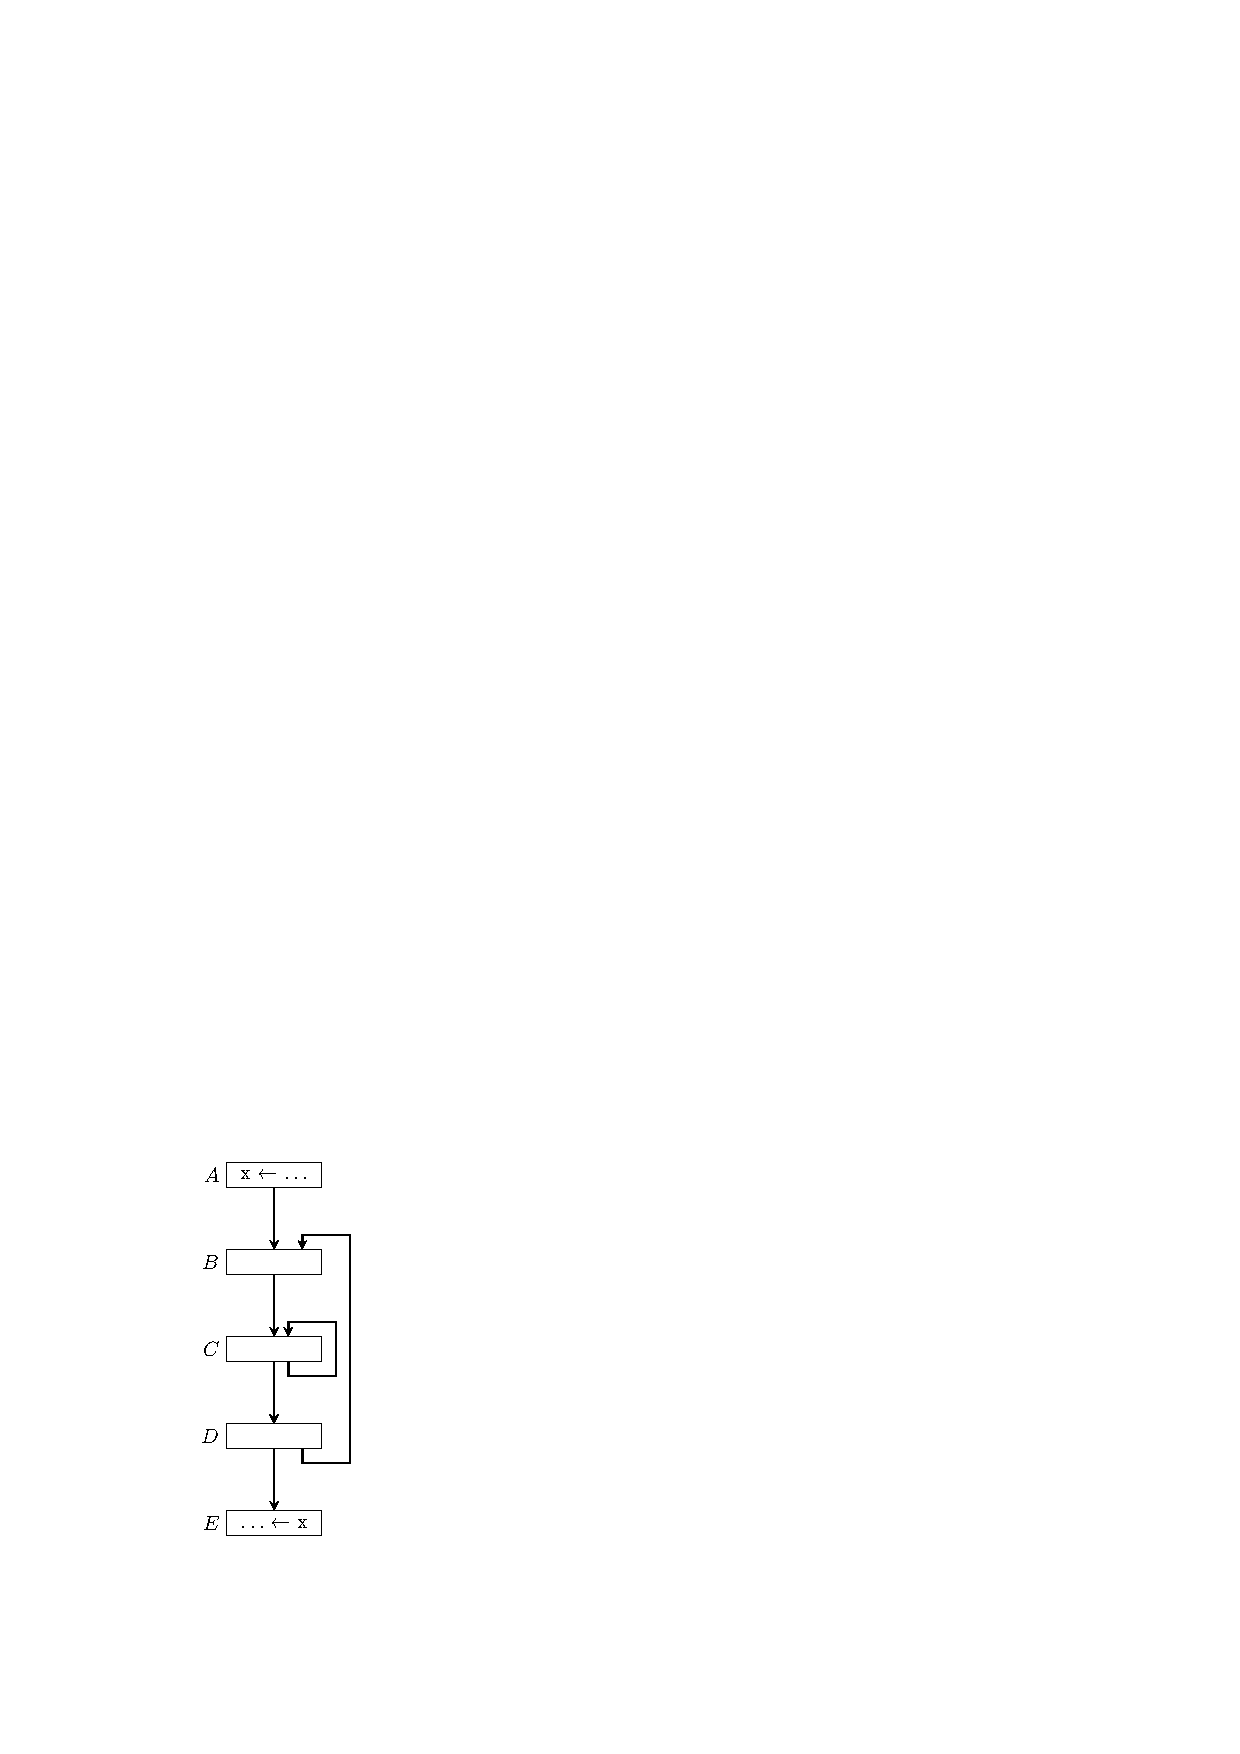
\includegraphics{phi_opt_orig.pdf}
		}
		\qquad
		\subfloat[Unnecessary \phifuns placed] {
			\label{fig:unn_phi_left}
			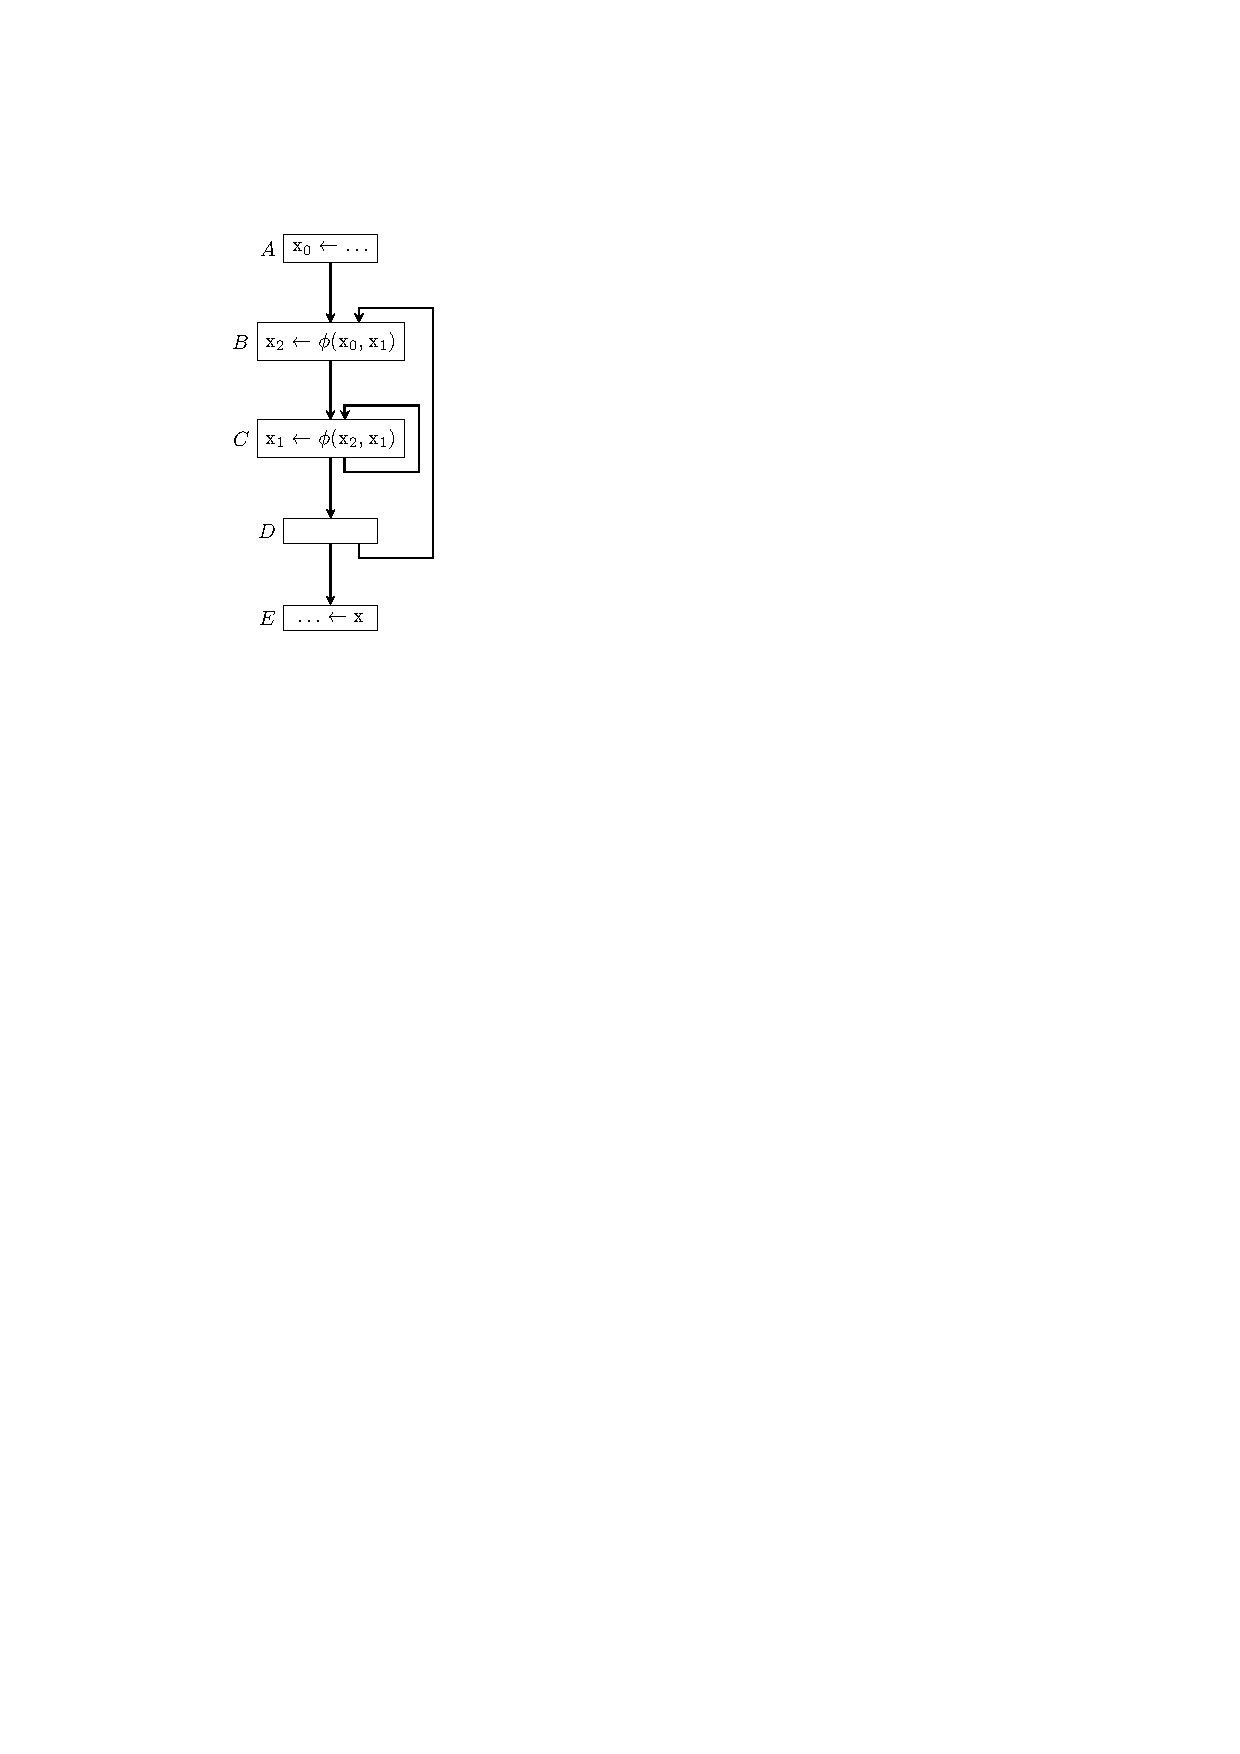
\includegraphics{phi_opt_unn.pdf}
		}
	\end{center}
	\caption{Removal of unnecessary \phifuns}
	\label{fig:phiopt}
\end{figure}
We look for a definition of $\var x$ from block~$E$.
If Algorithm~\ref{alg:ssaconstr_click} considers the blocks in a unfavorable order, e.g.~$D,C,B,A,D,C$, some unnecessary \phifuns can not be removed by \verb|phi_necessary|, as shown in Figure~\ref{fig:unn_phi_left}.
While the \phifun in block~$C$ can be eliminated by the local criterion applied by \verb|phi_necessary|, the \phifun in block~$B$ remains. 
This is, because the depth-first search carried out by \verb|find_def_from_begin| will not visit block~$B$ a second time.
To remove the remaining \phifuns, the local criterion can be iteratively applied to all placed \phifuns until a fixpoint is reached. 
For reducible control flow, this then produces the minimal number of placed \phifuns. 
The classical $(\ast)$-graph in Figure~\ref{fig:astgraph} illustrates that this does not hold for the irreducible case:
\begin{figure}[htbp]
	\begin{center}
		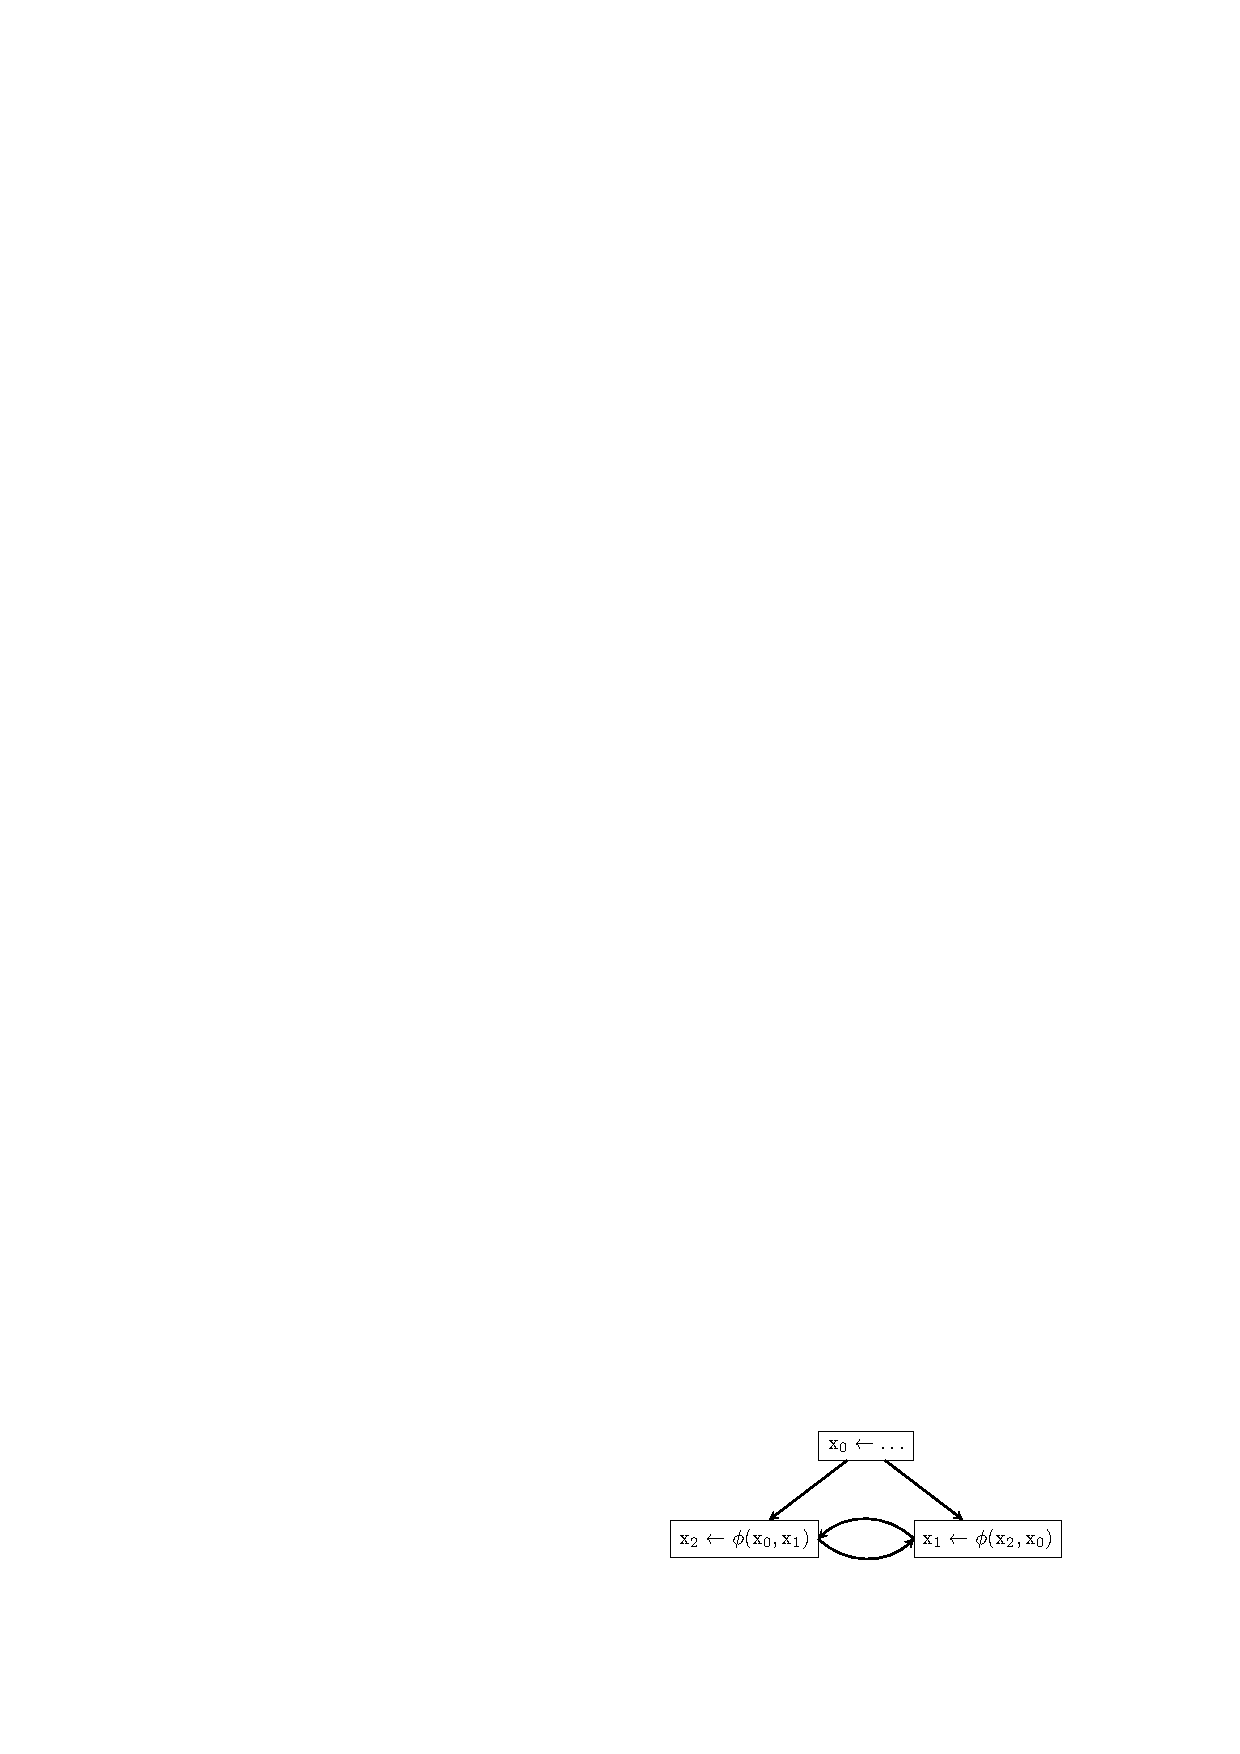
\includegraphics{ast_graph.pdf}
		\caption{The irreducible $(\ast)$-Graph}
		\label{fig:astgraph}
	\end{center}
\end{figure}


\section{Conclusions}

Some optimizations, such as loop unrolling or live-range splitting destroy the single-assignment property of the SSA form.
In this chapter we presented two generic algorithms to reconstruct SSA.
The algorithms are independent of the transformation that violated SSA and can be used as a black box:
For every variable for which SSA was violated, a routine is called that restores SSA.
Both algorithms rely on computed def-use chains because they traverse all uses from a SSA variable to find suitable definitions.
However, both algorithms differ in their prerequisites and their runtime behavior:
\begin{enumerate}
	\item 
		The first one~\cite{Choi:1996ji} is based on the iterated dominance frontiers like the classical SSA construction algorithm by Cytron et al.~\cite{cytron:1991:ssa}.
		Hence, it is less suited for optimizations that also change the flow of control since that would require recomputing the iterated dominance frontiers.
		On the other hand, by using the iterated dominance frontiers, the algorithm can find the reaching definitions quickly by scanning the dominance tree upwards.
		Furthermore, one could also envision applying incremental algorithms to construct the dominance tree~\cite{Ramalingam:1994iq,Sreedhar:1995:ICD:202529.202531} and the dominance frontier~\cite{Sreedhar:1996:NFE:231379.231434} to account for changes in the control flow. 
		this has not yet been done and no practical experiences have been reported so far.
	\item 
		The second algorithm does not depend on additional analysis information such as iterated dominance frontiers or the dominance tree.
		Thus, it is well suited for transformations that change the CFG because no information needs to be recomputed.
		On the other hand, it might find the reaching definitions slower than the first one because they are searched by a depth-first search in the CFG.
\end{enumerate}
Both approaches construct \emph{pruned} SSA (TODO: cite other chapter), i.e., no \phifun is dead. 
The first approach produces minimal SSA by the very same arguments Cytron et al.~\cite{cytron:1991:ssa} give.
The second one does only produce minimal SSA (in the sense of Cytron) in the case of reducible control flow. 
This follows from the iterative application of the function \verb|phi_necessary| which implements the two simplification rules presented by Aycock and Horspool~\cite{Aycock_Horspool_2000}.
They show that the iterative application of both rules yields minimal SSA on reducible graphs. 
These two local rules can be extended to a non-local one which then has to find strongly connected $\phi$-components that all refer to the same exterior variable.
Such a non-local check also eliminates unnecessary \phifuns in the irreducible case.

